\subsection{www.cam.ac.uk}

En esta ocasión se envió un paquete ICMP con destino hacia la URL \textit{www.cam.ac.uk}, donde está hosteado el sitio de la Universidad de Cambridge en el Reino Unido. Con el fin de obtener los nodos distinguidos, posteriormente se calculo el Z-Score en base a los resultados obtenidos con la herramienta implementada para este trabajo práctico.
En esta primera figura se puede ver el viaje que realizó el paquete hasta arribar a su destino, deduciendo la ubicación geográfica de los routers intermedios a partir de sus direcciones IP.

\begin{figure}[H]
  \centering	
	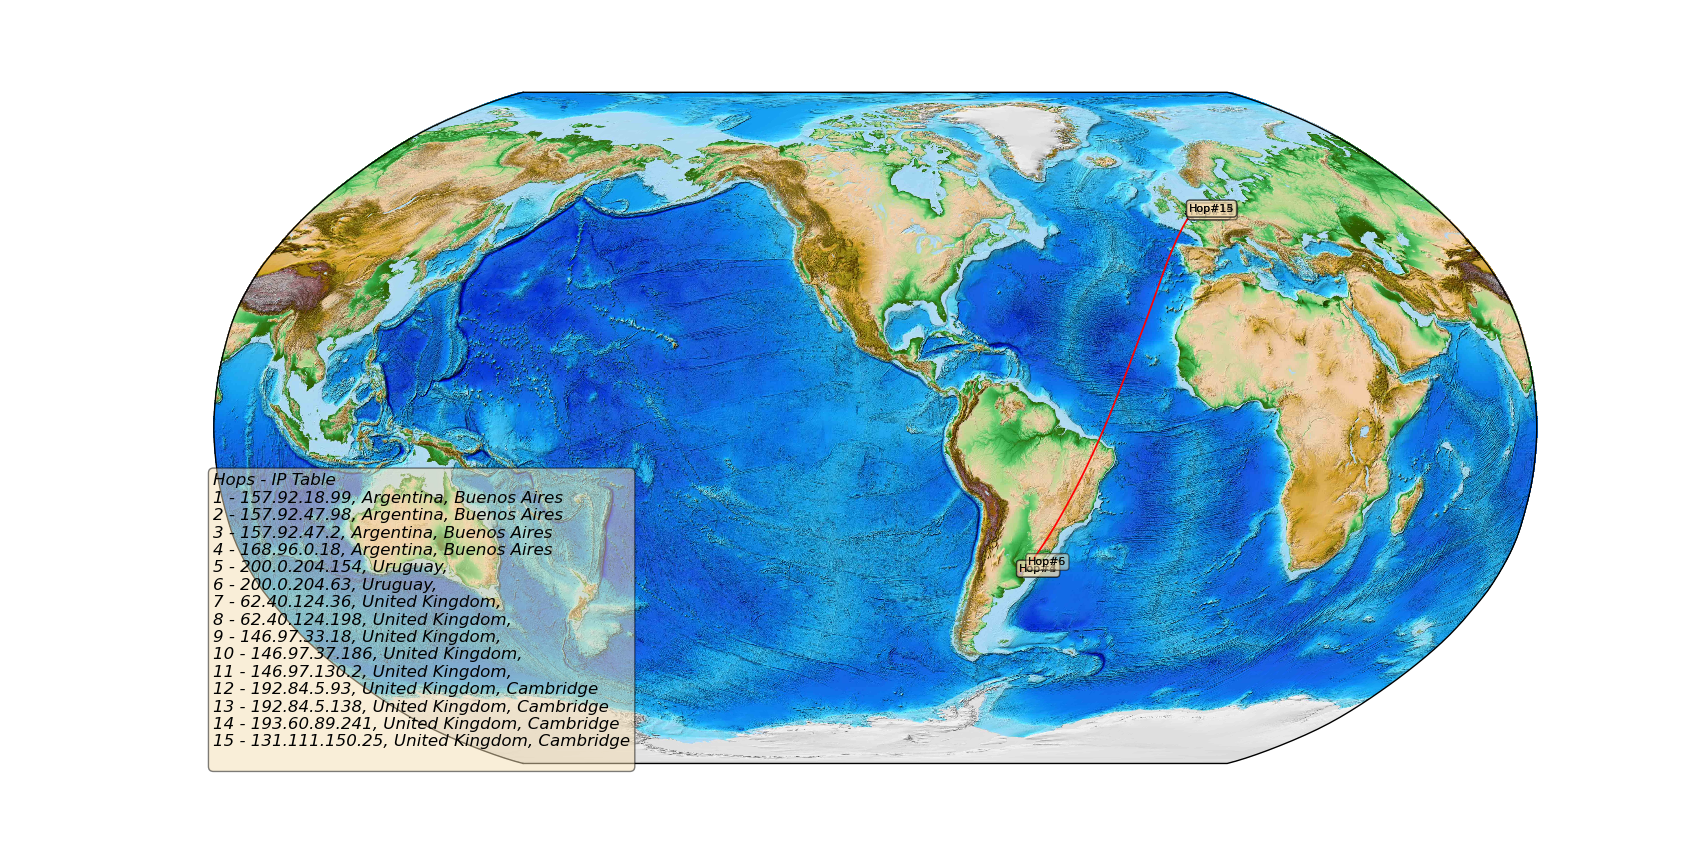
\includegraphics[scale=0.3]{../cambridge-experiment/figure_1.png}
  \caption{Planisferio donde se puede ver el realizado por el paquete en rojo.}
	\label{fig:histo-src-sitiotrabajo}
\end{figure}

En los siguientes gráficos se hallan los valores asociados a los \textit{Round Trip Time} que se estimaron entre cada uno de los nodos. En el primero de ellos se muestra el \textit{RTT} entre dos nodos consecutivos, mientras que en el segundo se puede apreciar el acumulado de estos a medida que el paquete se acerca al destino.

\begin{figure}[H]
  \centering	
	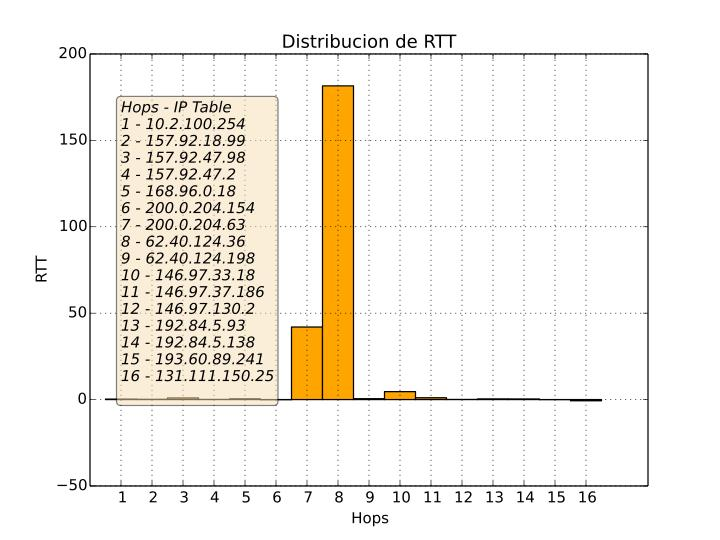
\includegraphics[scale=0.3]{../cambridge-experiment/bar_rtt.jpeg}
  \caption{RTT entre dos router consecutivos medido en milisegundos.}
	\label{fig:histo-src-sitiotrabajo}
\end{figure}

\begin{figure}[H]
  \centering	
	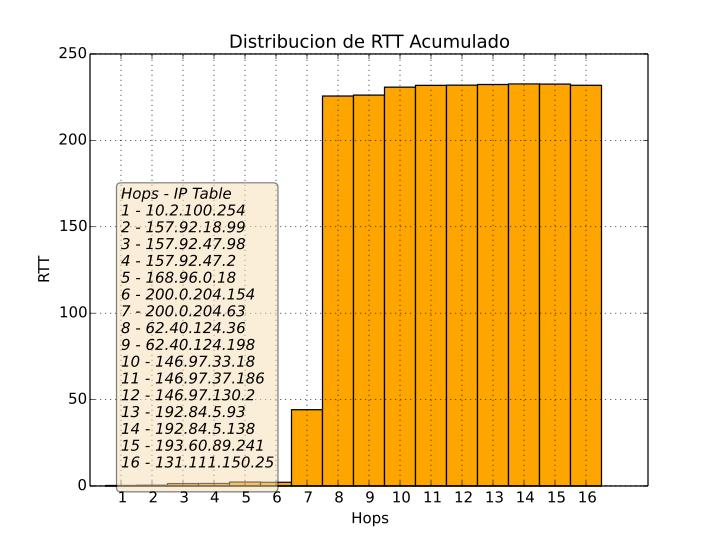
\includegraphics[scale=0.3]{../cambridge-experiment/bar_rtt_acum.jpeg}
  \caption{RTT acumulado del paquete a medida que avanza en su camino hacia la Universidad de Cambridge.}
	\label{fig:histo-src-sitiotrabajo}
\end{figure}

Finalmente, los resultados obtenidos por el Z-Score permiten distinguir a los saltos de mayor importancia en el trayecto, como era de esperarse estos están relacionados con el del salto transoceánico que se realiza entre Uruguay y el Reino Unido.

\begin{figure}[H]
  \centering	
	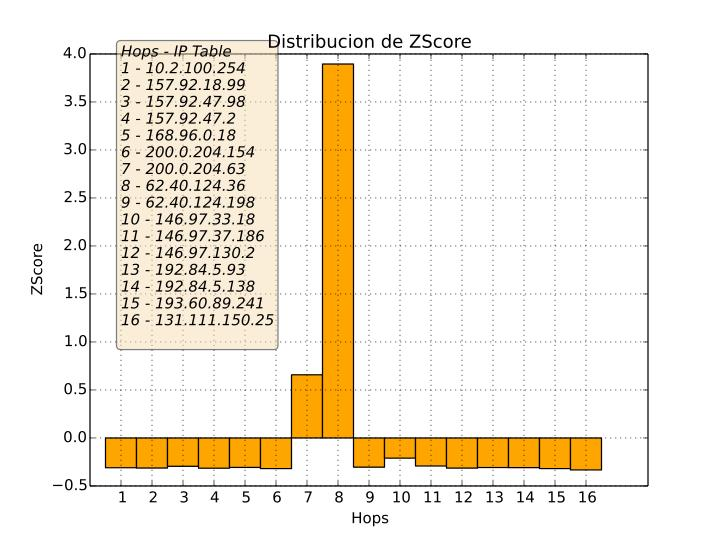
\includegraphics[scale=0.3]{../cambridge-experiment/bar_z_score.jpeg}
  \caption{Z-Score para cada uno de los saltos.}
	\label{fig:histo-src-sitiotrabajo}
\end{figure}
